\documentclass{ExamCUNY}
\usepackage{mathrsfs}
\usepackage{stix}
\usepackage{pgffor}
\usepackage{bm}
\usepackage{microtype}
\usepackage{nicematrix}
\usepackage{booktabs}
\usepackage{mathtools}
\usepackage{tikz}
\usetikzlibrary{calc, 3d}


\usepackage{tabstackengine}
\TABstackMath
\TABbinary



\ExamNumber{2}%
\CourseName{Probability and Statistics for Computer Science}
\CourseNumber{217}
\InstructorName{Alex Washburn}
\DueDateYear{2023}
\DueDateMonth{11}
\DueDateDay{07}


\newcommand{\?}{\stackrel{?}{=}}
\newcommand{\R}[2]{\ensuremath{\World{#1}\mathrel{R}\World{#2}}\xspace}
\newcommand{\Tr}[2]{\ensuremath{\tau\Parens{#1,\,#2}\xspace}}
\newcommand{\T}[1]{\ensuremath{\tau\Parens{#1}\xspace}}
\newcommand{\Prob}[1]{\ensuremath{P\Parens{#1}}\xspace}
\newcommand{\ProbGiven}[2]{\ensuremath{P\Parens{#1\,|\,#2}}\xspace}
\newcommand{\Event}[1]{\ensuremath{\bm{\mathsf{#1}}}\xspace}
\newcommand{\RandVar}[1]{\ensuremath{\mathbf{#1}}\xspace}
\newcommand{\DistMap}[2]{~#1&\mapsto~~#2\\}
\newcommand{\DistCondition}[2]{~#1&\text{\normalfont iff}~~#2\\}

\newcommand{\Hint}[1]{\textit{\textls{Hint:}~#1}}

\newcommand{\One}{\ensuremath{\textbf{1}}\xspace}

\newcommand{\EquivGrid}{\ensuremath{~\;\;\equiv\quad}\xspace}

\newcommand{\Coin}[1]{\ensuremath{\mathbf{C}_{#1}}\xspace}
\newcommand{\CoinBiased}[1]{\ensuremath{\mathscr{C}_{#1}}\xspace}
\newcommand{\Heads}{\ensuremath{\mathtt{H}}\xspace}
\newcommand{\Tails}{\ensuremath{\mathtt{T}}\xspace}

\newcommand{\Die}[1]{\ensuremath{\mathbf{D}_{#1}}\xspace}
\newcommand{\Above}[1]{\ensuremath{\overline{#1}}\xspace}
\newcommand{\Below}[1]{\ensuremath{\underline{#1}}\xspace}
\newcommand{\Num}[1]{\ensuremath{\mathbb{#1}}\xspace}
\newcommand{\NumA}[1]{\ensuremath{\overline{\Num{#1}}}\xspace}
\newcommand{\NumB}[1]{\ensuremath{\underline{\Num{#1}}}\xspace}

\newcommand{\Deck}{\ensuremath{\bm{\mathcal{D}}}\xspace}
\newcommand{\CardSuits}{\ensuremath{\bm{\mathcal{S}}}\xspace}
\newcommand{\CardRanks}{\ensuremath{\bm{\mathcal{R}}}\xspace}
\newcommand{\CardRank}[1]{\ensuremath{\text{\textsf{\textbf{#1}}}}\xspace}


\newcommand{\Countermodel}[4]{%
\textbf{Countermodel} $\mathcal{K}$ in #1:%
\begin{itemize}%
\item \ensuremath{W = \SetNote{\World{0}%
\foreach \n in {1,...,#2}{,~\World{\n}}%
}}%
\item \ensuremath{\mathrel{R}~=~#3}%
\item #4%
\end{itemize}%
}

\begin{document}
\CoverPage%

\newcommand{\BulletLong}[3]{\hspace*{4mm}\ensuremath{\Parens{\Event{#1}}}:\hspace*{2mm}#2\[#3\]\\[5mm]}
\newcommand{\BulletLine}[3]{\hspace*{4mm}\ensuremath{\Parens{\Event{#1}}}:\hspace*{2mm}#2\hfill\ensuremath{#3}\\[5mm]}
\newcommand{\Bullet}[2]{\hspace*{4mm}\ensuremath{\Parens{\Event{#1}}}:\hspace*{2mm}#2\\[5mm]}

\newcommand{\True}{\ensuremath{\bm{\mathtt{True}}}\xspace}
\newcommand{\False}{\ensuremath{\bm{\mathtt{False}}}\xspace}

\newcommand{\TrueFalse}[1]{\ensuremath{\True\;\oplus\;\False\;\colon~~{#1}}}
\newcommand{\TrueFALSE}[1]{\ensuremath{\True\;\oplus\;\underline{\False}\;\colon~~{#1}}}
\newcommand{\TRUEFalse}[1]{\ensuremath{\underline{\True}\;\oplus\;\False\;\colon~~{#1}}}

\newcommand{\SupportFalsify}[1]{\ensuremath{\mathtt{Support}\;\oplus\;\mathtt{Falsify}\;\colon~~{#1}}}
\newcommand{\SupportFALSIFY}[1]{\ensuremath{\mathtt{Support}\;\oplus\;\underline{\mathtt{Falsify}}\;\colon~~{#1}}}

\newcommand{\Bc}{\cellcolor{blue!20}}



\newcommand{\Reals}{\ensuremath{\mathbb{R}}\xspace}
\newcommand{\PMF}[2]{%
\expandafter\ifx\expandafter\relax%
\detokenize{#2}\relax\ensuremath{\rho_{{\textstyle\mathstrut}\RandVar{#1}}}\xspace\else\ensuremath{\rho_{{\textstyle\mathstrut}\RandVar{#1}}\Parens{#2}}\xspace\fi}

\newcommand{\PDF}[2]{%
\expandafter\ifx\expandafter\relax%
\detokenize{#2}\relax\ensuremath{\mathit{f}_{{\textstyle\mathstrut}\RandVar{#1}}}\xspace\else\ensuremath{\mathit{f}_{\RandVar{{\textstyle\mathstrut}#1}}\Parens{#2}}\xspace\fi}

\newcommand{\Expect}[1]{\ensuremath{\mathbb{E}\left[\,#1\,\right]}\xspace}
\newcommand{\Variance}[1]{\ensuremath{\mathtt{Var}\Parens{#1}}\xspace}

%%%%%%%%%%%%%
% Instructions
\newcommand{\Q}[1]{\ensuremath{\textbf{Question #1}}\xspace}

\clearpage%                                                                                                                                                                                           
\newgeometry{bottom=20mm,left=20mm,right=20mm,top=20mm}%  
\begin{center}
{\Huge \underline{Examination Instructions}}
\end{center}
~\vspace*{5mm}
{\Large
\begin{itemize}
\item Read each question carefully, preferably twice.
\item If you do not understand a question, raise your hand and ask for clarification.
\item There are no ``trick questions.''\\
The most straight-forward interpretation of the problem statement is likely the correct interpretation.
\item Show as much of your work and thought process as possible.\\
Partial credit will be given for partially correct answers.
\item I am looking to \emph{give} credit for correctness, not \emph{deduct} credit for mistakes.\\
It is \emph{always better} to be more verbose than to be terse, since you will receive full credit as long some of your solution correctly conveys the answer.
\vspace*{5cm}
\begin{center}
{\Huge \underline{Examination Scoring}}
\end{center}
\begin{align*}
\textit{\textbf{Final Score}} &= \Q{1}\\
&\,+ \Q{2}\\
&\,+ \Q{3}\\
&\,+ \textsc{Best~2~out~of~3}\\
&~\Parens{\Q{4},\,\Q{5},\,\Q{6}}
\end{align*}
\end{itemize}
}



\newcommand{\ExamObject}[2]{%
{\Large \underline{\textbf{|~#1}}}\\[5mm]%
{\Large #2}\\[5mm]%
}

%%%%%%%%%%%%%
% Combinatorial Objects

\clearpage%                                                                                                                                                                                          

\Problem{20}{Definitions}{%
Describe to the best of your ability the definition of each probability theory concept.
You may use the English language, mathematical notation, or some combination of both.
}

\SubProblem{5}{Probability Mass Function (PMF) of a random variable \RandVar{X}}
A function from $\PMF{X}{}: \Reals \mapsto \IndexRange{0}{1}$  which outputs the probability that the input value was measured from the observation of the \emph{discrete} sample space.
\[
\PMF{X}{} = \Prob{\RandVar{X} = x} = \Prob{\SetNote{\RandVar{X}(\omega)=x~|~\omega \in \Omega})}
\]
\vfill


\SubProblem{5}{PDF Total Probability Theorem}
For all random variables $\RandVar{X}$, the probabilities of all possible inputs to $\PDF{X}{}$ will total to 1.
\[
1 = \Prob{\Omega} = \int_{-\infty}^{\infty}\; \PDF{X}{x}dx
\]
\vfill


\SubProblem{5}{Expectation of a \emph{discrete} random variable \RandVar{X}}
The expectation is mean (average) value of measuring a \emph{discrete} random variable \RandVar{X}.
\[
\Expect{\RandVar{X}} = \sum\limits_{x}\; x*\PMF{X}{x}
\]
\vfill


\SubProblem{5}{Standard Deviation of a random variable \RandVar{X}}
The standard deviation of a random variable \RandVar{X}, denoted as $\sigma_{\RandVar{X}}$, is a measure of dispersion;\\how far a set of numbers is spread out from their mean value.\\[2mm]
The standard deviation is defined as the square root of the variance.
\[
\sigma_{\RandVar{X}}^2 = \Variance{\RandVar{X}}
\]
\vfill


\Problem{20}{True or False}{%
Decide whether each statement is \texttt{True} or \texttt{False},\\
 based on the probability mass functions for random variables \RandVar{X} and \RandVar{Y}:
\begin{equation*}
\PMF{X}{}=
\begin{cases}
\DistMap{1}{\frac{4}{10}}
\DistMap{2}{\frac{3}{10}}
\DistMap{3}{\frac{2}{10}}
\DistMap{4}{\frac{1}{10}}
\end{cases}\hspace*{3cm}
\PMF{Y}{}=
\begin{cases}
\DistMap{1}{\frac{1}{30}}
\DistMap{2}{\frac{4}{30}}
\DistMap{3}{\frac{9}{30}}
\DistMap{4}{\frac{16}{30}}
\end{cases}
\end{equation*}
}

\SubProblem{4}{%
\TrueFalse{2 \,=\, \Expect{\RandVar{X}}}}
\[
\underline{\True}\qquad2 \,=\, \Expect{\RandVar{X}} = \sum_{i=1}^{4} i\times\PMF{X}{i} = \frac{1 \times 4}{10} + \frac{3 \times 2}{10} + \frac{2 \times 3}{10} + \frac{4 \times 1}{10} = \frac{4 + 6 + 6 + 4}{10} = \frac{20}{10}
\]
\vfill


\SubProblem{4}{%
\TrueFalse{\pi \,=\, \Expect{\pi \times \RandVar{X} - \pi}}}
\[
\underline{\True}\qquad\pi \,=\, \Expect{\pi \times \RandVar{X} - \pi} = \pi \times \Expect{\RandVar{X}} - \pi = \pi \times 2 - \pi
\]
\vfill


\SubProblem{4}{%
\TrueFalse{\pi \,\ge\, \Expect{\RandVar{Y}}}}
\[
\underline{\False}\qquad\pi \,\ge\, \Expect{\RandVar{Y}} = \sum_{i=1}^{4} i\times\PMF{Y}{i} = \frac{1 \times 1}{30} + \frac{2 \times 4}{30} + \frac{3 \times 9}{30} + \frac{4 \times 16}{30} = \frac{1 + 8 + 27 + 64}{30} = \frac{100}{30} = 3.\overline{3}
\]
\vfill


\SubProblem{4}{%
\TrueFalse{\pi \,\ge\, \Variance{\frac{1}{10} \times \RandVar{Y} + 5040}}}
\[
\underline{\True}\qquad\pi \,\ge\, \Variance{\frac{1}{10} \times \RandVar{Y} + 5040} = \frac{1}{10^2}\times \Variance{\RandVar{Y}} = \frac{1}{10^2}\times\Parens{\Expect{Y^2} - \Expect{Y}^2} = \frac{1}{10^2}\times\Parens{\frac{59}{5} - \frac{100}{30}} = 0.118 - 0.03\overline{3}
\]
\vfill


\SubProblem{4}{%
\TrueFalse{\Expect{3 \times \RandVar{X} + 2} \;=\; \Expect{3 \times \RandVar{Y} - 2}}}
\[
\underline{\True}\qquad\Expect{3 \times \RandVar{X} + 2} = \Expect{3 \times \RandVar{Y} - 2} \;\equiv\; 3 \times \Expect{X} + 2 = 2 \times \Expect{Y} - 2 \;\equiv\; 3 \times 2 + 2 = 3 \times 3.\overline{3} - 2 \;\equiv\; 8 = 8
\]
\vfill


\Problem{20}{Support or Falsify}{%
Consider each statement and regarding the following\\\emph{joint} probability mass function \PMF{X,Y}{} and either:\\[5mm]
\begin{equation*}
\linespread{3em}
\PMF{X,Y}{}=\begin{cases}%
\begin{smallmatrix}%
~3~\vert &~\frac{1}{68} & ~\frac{2}{68} & ~\frac{25}{68} \\~~~\vert&&&\\%
~2~\vert & ~\frac{2}{68} &  ~\frac{4}{68} & ~\frac{16}{68} \\~~~\vert&&&\\%
~1~\vert & ~\frac{3}{68} &  ~\frac{6}{68} & ~\frac{ 9}{68} \\\makebox[0.55cm]{\rule{1cm}{0.5pt}}\vert&\makebox[0.67cm]{\rule{1cm}{0.5pt}}&\makebox[0.67cm]{\rule{1cm}{0.5pt}}&\makebox[0.67cm]{\rule{1cm}{0.5pt}}\\%
\frac{\RandVar{Y}}{\RandVar{X}}\;\vert& ~1 & ~2 & ~3%
\end{smallmatrix}
\end{cases}
\end{equation*}
\large
\Bullet{Support}{State that it is $\mathtt{True}$. Explain the reason why you believe that is the case. If you feel capable of providing a proof or a sketch/outline of a proof, please do so}
\Bullet{Falsify}{State that it is $\mathtt{False}$. Explain the reason why you believe that is the case. If you have a counterexample which shows that the statement is false, please provide it.}
}
 
\SubProblem{5}{\SupportFalsify{\Expect{\PMF{X}{}}~<~\Expect{\PMF{Y}{}}}}
\[
\underline{\False}\qquad\sum_{i=1}^{3} i\times\PMF{X}{i} \not< \sum_{i=1}^{3} i\times\PMF{Y}{i} \;\equiv\; \frac{1\times6}{68} + \frac{2\times12}{68} + \frac{3\times50}{68} \not< \frac{1\times18}{68} + \frac{2\times22}{68} + \frac{3\times28}{68} \;\equiv\; \frac{180}{68} \not< \frac{146}{68}
\]
\vfill


\SubProblem{5}{\SupportFalsify{\forall x, y\quad\PMF{X\vert Y}{x\,\vert\,2}~<~\PMF{Y\vert X}{y\,\vert\,2}}}
\[
\underline{\False}\qquad\exists x, y \text{~such that~}\PMF{X\vert Y}{x\,\vert\,2}~\not<~\PMF{Y\vert X}{y\,\vert\,2}\quad \text{~counter-example~} \PMF{X,Y}{3,2} \not< \PMF{X,Y}{2,1} \equiv \frac{16}{68} \not< \frac{6}{68} 
\]
\vfill


\SubProblem{5}{\SupportFalsify{\frac{1}{2}~<~\Prob{\RandVar{X} \;<\; \RandVar{Y}}}}
\[
\underline{\False}\qquad\frac{1}{2}~<~\Prob{\RandVar{X} \;<\; \RandVar{Y}} = \sum_{i=1}^{3} \sum_{j=1}^{i - 1} \PMF{X,Y}{j,\,i} = \frac{6}{68} + \frac{9}{68} + \frac{16}{68} = \frac{31}{68} \approx 0.456
\]
\vfill

\SubProblem{5}{\SupportFalsify{\frac{1}{2}~<~\Prob{\RandVar{X} \;=\; 3}}}
\[
\underline{\True}\qquad\frac{1}{2}~<~\Prob{\RandVar{X} \;=\; 3} = \frac{9}{68} + \frac{16}{68} + \frac{25}{68}= \frac{50}{68}
\]
\vfill


\Problem{20}{Problem 1}{%
Alice flips a coin $n$ times.
She counts $k$ heads occurring from the $n$ coin flips.
In order to determine the probability $\Prob{\Heads} = q$ that a coin flip produces \Heads, Alice repeats the experiment $1,000,000$ times.
The plot of outcomes from all of Alice's experiments is shown below. %
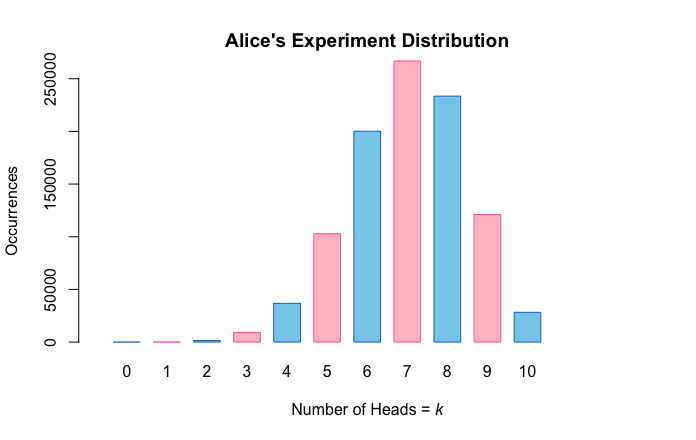
\includegraphics[width=\textwidth]{Distribution-Alice.png}}

\SubProblem{10}{How many coin flips did Alice make in each experiment; i.e. what is the value of $n$?}
The number of \Heads measured range from \NumericRange{0}{10} in the presented plot.
Therefore, Alice flipped the coin $10$  times in each experiment, because $10$ was the largest measurement.
\vfill

\SubProblem{10}{What is the probability of getting heads Alice flips her coin; i.e. what is $\Prob{\Heads} = q$?}
The measurement of $7 \Heads$ occurrence most often (highest bar).
There were $10$ coin flips in each experiment.
Therefore, the probability of s single coin flip being \Heads is $\frac{7}{10}$.
\vfill


\Problem{20}{Problem 2}{%
Bob flips a coin as many times as necessary until a heads \Heads occurs.
He notes the number of flips required for \Heads to occur.
In order to determine the probability $\Prob{\Heads} = q$ that a coin flip produces \Heads, Bob repeats the experiment $1,000,000$ times.
The plot of outcomes from all of Bob's experiments is shown below. %
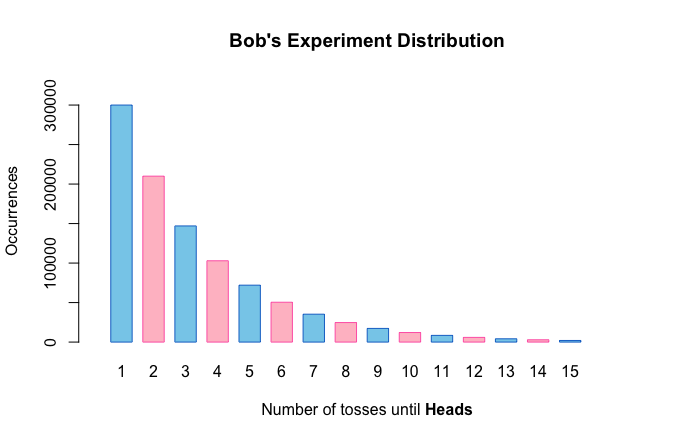
\includegraphics[width=\textwidth]{Distribution-Bob.png}}

\SubProblem{10}{What is the probability of heads when flipping Bob's coin; i.e. what is $\Prob{\Heads} = q$?}
The probability of \Heads occurring on the first coin flip is equal to the relative height of the bar for $1$.
Bob repeated the experiment $1,000,000$  times and observed the first coin flip resulted in \Heads $300,000$ times.
\[
\text{Therefore~} \Prob{\Heads} = q = \frac{300,000}{1,000,000} = \frac{3}{10} = 0.3
\]
\vfill

\SubProblem{10}{On average, how many coin flips are required for a \Heads to occur; i.e. $\Expect{\RandVar{X}}$?}
The expectation of a geometric distribution is $\frac{1}{q}$.
Therefore, on average it takes the following number of coin flips are required for a \Heads to occur:
\[
\Expect{\RandVar{X}} = \frac{1}{q} = \frac{1}{\frac{3}{10}} = \frac{10}{3} = 3.\overline{3}
\]
\vfill

\Problem{20}{Problem 3}{%
Ross is a paleontologist with the Museum of Prehistoric History and just unearthed a mass grave of $100!$ T-Rex fossils on his fieldwork expedition!
Ross diligently takes measurements of all fossils recovered.
Later Ross looks over his measurements of all $100$ T-Rex femur lengths and plots the number of femurs with the same length as shown below. %
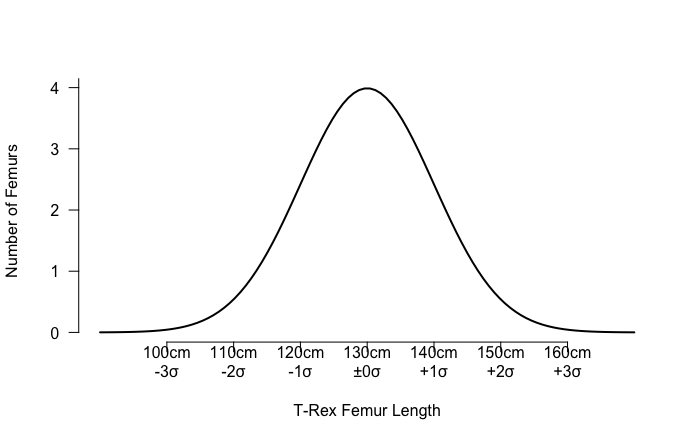
\includegraphics[width=\textwidth]{Distribution-Ross.png}}

\SubProblem{10}{What is the average femur length Ross found?}
This is a Normal Distribution.
Hence, the mean (average) value is simply the highest point on the curve.
Therefore the average femur length is $130\text{cm}$.
\vfill

\SubProblem{10}{What is the standard deviation of the femur lengths Ross found?}
This is a Normal Distribution.
Therefore the standard deviation is the difference between the mean value \Parens{\mu = \pm0\sigma} and the square root of the variance \Parens{\pm1\sigma}.
Therefore the standard deviation of femur length is:
\[
\mu \pm1\sigma = 130\text{cm} - 120\text{cm} = 10\text{cm}
\]
\vfill


\end{document}
